\section{Enabling Technologies}

A range of technologies developed over several years have enabled the evolution of NFV and Edge Computing. This seections briefly describes and compares the technologies that led to the development of MEC and its parallel technology NFV.

These technologies can be grouped into 4 different planes based on their functionalities.

\begin{enumerate}
    \item Data Plane
	\begin{itemize}
	    \item Follows the forwarding logic and responsible for physically moving the packets in the network.
        \end{itemize}
    \item Control Plane
	\begin{itemize}
	    \item Computes the forwarding logic as required by the other planes and programs them to the Data plane and monitors the data plane.
        \end{itemize}
    \item Management Plane
	\begin{itemize}
	    \item Responsible for orchestration and management of resources as required by the services.
	\end{itemize}
    \item Application Plane
	\begin{itemize}
	    \item Makes use of the services through Service Abstraction and APIs from Management to deliver end-user applications.
	\end{itemize}
\end{enumerate}

These planes are depicted in the figure below in Figure 6.

\begin{figure}
	\centering
        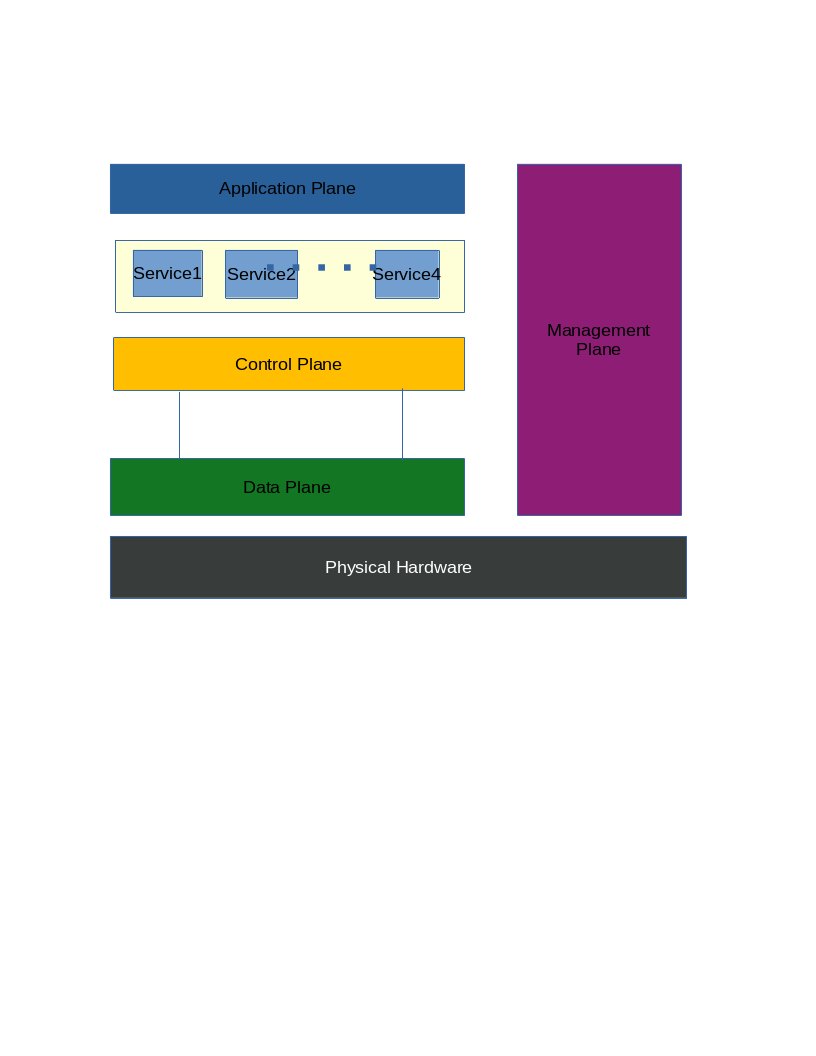
\includegraphics[width=0.7\textwidth]{planes_of_computing}
	\label{fig:figure6}
	\caption{Planes of NFV and MEC Architectures}
\end{figure}

The architecture also evolves into multiple business models as envisaged by the NIST Cloud Computing group

\begin{enumerate}
    \item Infrastructure As A Service
    \item Platform as a Service
    \item Software As A Service
\end{enumerate}
